\documentclass[12pt, a4paper]{article}
\usepackage[utf8]{inputenc}
\usepackage{polski}
\usepackage{hyperref}
\usepackage{graphicx}
\usepackage{algorithm}
\usepackage{algpseudocode}
\usepackage{amsmath}
\usepackage{amsfonts}
\usepackage{float}
\usepackage{geometry}
\title{\textbf{Porównanie klasycznej ewolucji różnicowej DE/rand z odmianą przesuwającą punkt środkowy DE/mid}}
\author{Adam Stelmaszczyk}
\date{\today}
\setlength{\parindent}{0in}
\renewcommand\refname{Referencje}

\def\C{{\rm C}\,}

\begin{document}
\maketitle

\begin{abstract}
W pracy porównano klasyczny algorytm ewolucji różnicowej DE/rand z jego odmianą DE/mid.
W części teoretycznej wyprowadzono parametry skalujące dla obydwu algorytmów. W części praktycznej
przeprowadzono szereg eksperymentów na 7 wybranych funkcjach z BBOB 2013 \cite{hansen}. DE/mid
okazał się lepszy na większości z nich.
\end{abstract}

\section{Część teoretyczna}

Klasyczna ewolucja różnicowa DE/rand oraz jej odmiana DE/mid różnią się jedynie operatorem mutacji.
W DE/rand/k, mutant $i$-tego osobnika w populacji $P$ o $n$ osobnikach powstaje w następujący sposób \cite{opara}:
\begin{equation} \label{eq:derand}
u_i = P_{i_1} + \frac{F}{\sqrt{k}}\sum\limits_{j=1}^k (P_{i_{2j}} - P_{i_{2j+1}}),
i \neq i_1 \neq i_2 \neq \dots \neq i_{2k+1}
\end{equation}

$k \in \mathbb{N}$ to liczba wektorów różnic. $F\in\mathbb{R}$ to parametr skalujący dla DE/rand/1. \\

W DE/mid/k mutant powstaje w podobny sposób:

\begin{equation} \label{eq:demid}
u_i' = m + F_m\sum\limits_{j=1}^k (P_{i_{2j}} - P_{i_{2j+1}}), 
i \neq i_1 \neq i_2 \neq \dots \neq i_{2k+1}, k \in \mathbb{N}
\end{equation}

Jedyną różnicą jest $m$, czyli punkt środkowy populacji:
\begin{equation} \label{eq:midpoint}
m = \frac{1}{n}\sum\limits_{j=1}^n P_j
\end{equation}

$F_m\in\mathbb{R}$ jest parametrem skalującym dla DE/mid, analogicznym do $F$ dla DE/rand. 
Żeby macierz kowariancji populacji w DE/mid/k była taka sama jak w DE/rand/k, 
macierz kowariancji mutanta $\C[u_i]$ musi być taka sama jak macierz kowariancji mutanta $\C[u_i']$.
Można to osiągnąć tak dobierając $F_m$, żeby było spełnione równanie:
\begin{equation} \label{eq:rownanie}
\C[u_i] = \C[u_i']
\end{equation}

Osobniki są liniowo niezależne od siebie, dlatego:
\begin{align*}
\C[u_i] \overset{(\ref{eq:derand})}{=} \C[P_{i_1} + \frac{F}{\sqrt{k}}\sum\limits_{j=1}^k (P_{i_{2j}} - P_{i_{2j+1}})] = \C[P_{i_1}] + \C[\frac{F}{\sqrt{k}}\sum\limits_{j=1}^k (P_{i_{2j}} - P_{i_{2j+1}})] \\
= \C[P_{i_1}] + \frac{F^2}{k}\C[\sum\limits_{j=1}^k (P_{i_{2j}} - P_{i_{2j+1}})] = \C[P_{i_1}] + \frac{F^2}{k}\C[\sum\limits_{j=2}^{2k+1} P_{i_{j}}]
\end{align*}

$\forall{i}\hspace{1mm}\C[P_i] = \C[P]$, ponieważ każdy osobnik ma taki sam rozkład prawdopodobieństwa. Zatem:
\begin{align*} 
\C[u_i] = \C[P_{i_1}] + \frac{F^2}{k}\C[\sum\limits_{j=2}^{2k+1} P_{i_{j}}] = \C[P] + \frac{F^2}{k}\C[\sum\limits_{j=2}^{2k+1} P] \\
= \C[P] + \frac{F^2}{k}2k\C[P] = \C[P] + 2F^2\C[P] = (1 + 2F^2)\C[P]
\end{align*}

Rozwijając prawą stronę równania (\ref{eq:rownanie}):
\begin{align*}
\C[u_i'] \overset{(\ref{eq:demid})}{=} \C[m + F_m\sum\limits_{j=1}^k (P_{i_{2j}} - P_{i_{2j+1}})] \\
\overset{(\ref{eq:midpoint})}{=} \C[\frac{1}{n}\sum\limits_{j=1}^n P_j] + F_m^2\C[\sum\limits_{j=1}^k (P_{i_{2j}} - P_{i_{2j+1}})] 
= \frac{1}{n}\C[P] + F_m^2\C[\sum\limits_{j=2}^{2k+1} P] = (\frac{1}{n} + 2kF_m^2)\C[P]
\end{align*}

Zatem $\C[u_i]$ = $(1 + 2F^2)\C[P]$ oraz $\C[u_i'] = (\frac{1}{n} + 2kF_m^2)\C[P]$. Podstawiając do (\ref{eq:rownanie}):
\begin{align*}
(1 + 2F^2)\C[P] = (\frac{1}{n} + 2kF_m^2)\C[P]
\end{align*}

Przy założeniu, że $\C[P] \neq 0$:
\begin{align*}
1 + 2F^2 = \frac{1}{n} + 2kF_m^2 \\
\frac{1 + 2F^2 - \frac{1}{n}}{2k} = F_m^2
\end{align*}
Obie strony są nieujemne, więc:
\begin{align} \label{eq:a}
F_m\ = \sqrt{\frac{1 + 2F^2 - \frac{1}{n}}{2k}}
\end{align}

Przyjmijmy $F=0.9$. Wówczas z (\ref{eq:a}) wynika, że: \\
$F_m \approx 1.14$ dla $k=1$ i $n\to\infty$. \\

W DE/mid/1, zamiast przesuwać losowo wybranego osobnika $P_i$, przesuwamy punkt środkowy.
Punkt środkowy jest mniej zmienny, 
tzn. norma macierzy kowariancji punktu środkowego jest mniejsza niż norma macierzy kowariancji dowolnego osobnika.
$\lim_{n\to\infty} \C[m] = 0$, natomiast $\C[P_i] = \C[P]$.
Dlatego DE/mid/1 potrzebuje większego współczynnika skalującego niż DE/rand/1. \\

W przypadku $k\to\infty$, zgodnie z centralnym twierdzeniem granicznym, wyrażenie $\sum\limits_{j=1}^k (P_{i_{2j}} - P_{i_{2j+1}})$ 
można traktować jak zmienną losową $v_\infty$ o rozkładzie $\mathcal{N}(0, \C[P])$. 
Wówczas równanie mutanta DE/rand/$\infty$ można zapisać jako:
\begin{align*}
u_i = P_{i_1} + F_\infty \cdot v_\infty
\end{align*}

Wyznaczmy $F_\infty$.
\begin{align*}
\C[u_i] = \C[P_{i_1} + F_\infty \cdot v_\infty] = \C[P] + 2F^2\C[P] \\
\C[P] + \C[F_\infty \cdot v_\infty] = \C[P] + 2F^2\C[P] \\
\C[F_\infty \cdot v_\infty] = 2F^2\C[P] \\
F_\infty^2 \C[P] = 2F^2\C[P] \\
F_\infty^2 = 2F^2 \\
F_\infty = \sqrt{2}F
\end{align*}

Równanie mutanta DE/mid/$\infty$ można zapisać podobnie:
\begin{align*}
u_i' = m + F_{\infty_m} \cdot v_\infty
\end{align*}

Wyznaczmy $F_{\infty_m}$.
\begin{align*}
\C[u_i'] = \C[m + F_{\infty_m} \cdot v_\infty] = \C[P] + 2F^2\C[P] \\
\C[m] + C[F_{\infty_m} \cdot v_\infty] = \C[P] + 2F^2\C[P] \\
\frac{C[P]}{n} + F_{\infty_m}^2 C[P] = \C[P] + 2F^2\C[P] \\
F_{\infty_m} = \sqrt{1 + 2F^2 - \frac{1}{n}}
\end{align*}

Tabela \ref{table:parametry} podsumowuje znalezione parametry skalujące.

\begin{table}[H]
\centering
\begin{tabular}{ l | c }
                 & parametr \\ \hline
DE/rand/1        & $F$ \\ 
DE/rand/k        & $\sqrt{\frac{2F^2}{2k}} = \frac{F}{\sqrt{k}}$ \\ 
DE/mid/k         & $\sqrt{\frac{1 + 2F^2 - \frac{1}{n}}{2k}}$ \\
DE/rand/$\infty$ & $\sqrt{2F^2} = \sqrt{2}F$ \\ 
DE/mid/$\infty$  & $\sqrt{1 + 2F^2 - \frac{1}{n}}$ \\
\end{tabular}
\caption{Parametry skalujące}
\label{table:parametry}
\end{table}

\section{Część praktyczna}

Zbadano 4 algorytmy:
\begin{enumerate}
\item DE/rand/1
\item DE/mid/1 
\item DE/rand/$\infty$ 
\item DE/mid/$\infty$ 
\end{enumerate}

Ekperymenty przeprowadzono na 7 funkcjach testowych o numerach 24, 110, 113, 116, 119, 122, 126 z BBOB 2013 \cite{hansen}, zaimplementowanych w języku C.
Funkcje testowe są wywoływane z Javy, w której napisano algorytmy oraz procedurę testującą.
Liczba wymiarów $D = 10$. Maksymalna liczba wywołań funkcji oceny $FEs = 10^6$. Rozmiar populacji $n = 100$. 
Jeśli algorytm nie znajdował minimum, wówczas w jednym uruchomieniu, na jednej funkcji, generował $10^4$ pokoleń.
Na każdej funkcji algorytm był niezależnie uruchamiany 100 razy, z każdego uruchomienia zapisywany był najlepszy wynik.
Parametry skalujące zgodne z tabelą \ref{table:parametry_liczbowe}, $F = 0.9$. Prawdopodobieństwo krzyżowania $Cr = 0.9$. \\

\begin{table}[H]
\centering
\begin{tabular}{ l | c }
                 & wartość \\ \hline
DE/rand/1        & $0.9$ \\ 
DE/mid/1         & $1.14...$ \\
DE/rand/$\infty$ & $1.27...$ \\ 
DE/mid/$\infty$  & $1.62...$\\
\end{tabular}
\caption{Wartości parametrów skalujących użyte w eksperymentach}
\label{table:parametry_liczbowe}
\end{table}

W celu porównania, wykreślano dystrybuanty empiryczne najlepszych wyników z każdego uruchomienia 
dla obu algorytmów na jednej funkcji. Wykresy przedstawiono poniżej.
Najlepszym wynikiem była najmniejsza odległość funkcji oceny osobnika od minimum.
Algorytm, którego dystrybuanta na wykresie przebiegała powyżej pozostałych, otrzymywał 3 punkty. 
Za drugie miejsce algorytm dostawał 2 punkty, za trzecie 1, za ostatnie 0. 
Jeśli dystrybuanty się przecinały, algorytmy zajmowały i-te miejsce ex aequo i dostawały punkty za i-te miejsce.
Przykładowo, na 110 funkcji DE/mid/1 i DE+/mid/1 wygrały, a DE/rand/1 i DE+/rand/1 zajęły trzecie miejsce.
Dostały następującą liczbę punktów, odpowiednio: 3, 3, 1, 1.
Wyniki przedstawia tabela \ref{table:compare}. \\ 

\begin{table}
\centering
\begin{tabular}{ l | c | c | c | c | c | c | c | c}
              & 24 & 110 & 113 & 116 & 119 & 122 & 126 & suma \\ \hline
DE/rand/1     & 3  & 1   & 0   & 0   & 1   & 3   & 0   & 8    \\ 
DE+/rand/1    & 3  & 1   & 1   & 1   & 1   & 3   & 3   & 13   \\ 
DE/mid/1      & 3  & 3   & 3   & 3   & 3   & 3   & 1   & 19   \\ 
DE+/mid/1     & 3  & 3   & 2   & 3   & 3   & 3   & 3   & 20   \\
\end{tabular}
\caption{Porównanie algorytmów}
\label{table:compare}
\end{table}

Para DE/mid/1 okazała się zdecydowanie lepsza niż DE/rand/1. Na 113, 116, 119, 122 i 126 funkcji DE/mid/1
znalazł minimum, podczas gdy DE/rand/1 nigdy się to nie udało. Ocenianie punktu środkowego zazwyczaj pomagało,
ale nie zawsze. DE+/rand/1 nigdy nie był gorszy niż DE/rand/1. Natomiast DE+/mid/1 przegrał
na 113 funkcji z DE/mid/1. Na pozostałych zazwyczaj sprawował się podobnie, raz wygrywając na funkcji 126.
Funkcje 24 oraz 122 okazały się nieprzydatne, ponieważ nie wykazały jednoznacznie przewagi żadnego z algorytmów. \\ 

\pagenumbering{gobble}

\begin{figure}
\centering
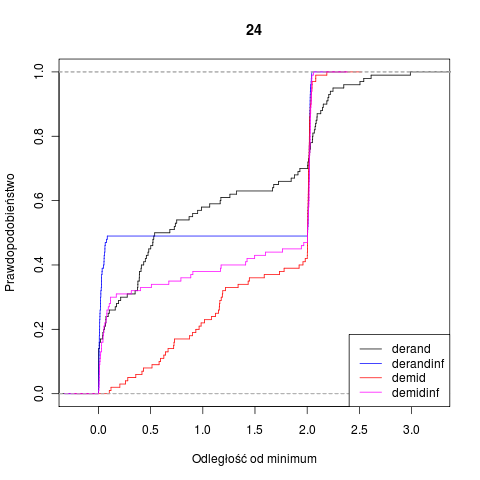
\includegraphics[scale=0.75]{../pngs/24.png} 
\includegraphics[scale=0.75]{../pngs/110.png}
\end{figure}

\begin{figure}
\centering
\includegraphics[scale=0.75]{../pngs/113.png}
\includegraphics[scale=0.75]{../pngs/116.png}
\end{figure}

\begin{figure}
\centering
\includegraphics[scale=0.75]{../pngs/119.png}
\includegraphics[scale=0.75]{../pngs/122.png}
\end{figure}

\begin{figure}
\centering
\includegraphics[scale=0.75]{../pngs/126.png}
\end{figure}

\bibliographystyle{plain}
\bibliography{references}

\end{document}